\documentclass{article}
\usepackage[utf8]{inputenc}
\usepackage{graphicx}
\usepackage{hyperref}
\usepackage{geometry}
\usepackage{fancyhdr}
\usepackage{titletoc}
\usepackage{lipsum}

% Define header and footer
\pagestyle{fancy}
\lhead{\footnotesize Project Report: Analyze Death Age Difference of Right Handers with Left Handers }
\rhead{}
\fancyfoot{}
\lfoot{\hrule \thepage}
\rfoot{\hrule \footnotesize MedTourEasy Project report, Hitesh M, Bengaluru} % Line and footer text
% ----------x-------------x----------------x-------------x--------------x--------------x-------------x----------
% Cover page content
\newcommand\coverpage{
    \thispagestyle{empty}
        \begin{center}
        \includegraphics[height=570pt]{logo.png}\\
        \vspace{1cm}
    \end{center}
    \clearpage
}



% ----------x-------------x----------------x-------------x--------------x--------------x-------------x----------
\newpage
\vspace{1cm}
\coverpage % Insert the cover page 
\newline
\begin{document}
\tableofcontents

% ----------x-------------x----------------x-------------x--------------x--------------x-------------x----------

\newpage
\section*{Acknowledgments}
\addcontentsline{toc}{section}{Acknowledgments}
\Large{I would also like to thank the team of MedTourEasy and my colleagues who made the working environment productive and very conducive. The traineeship opportunity that I had with MedTourEasy was a great change for learning and understanding the intricacies of the subject of Data Visualizations in Data Analytics; and also, for personal as well as professional development. I am very obliged for having a chance to interact with so many professionals who guided me throughout the traineeship project and made it a great learning curve for me. \\ \\ Firstly, I express my deepest gratitude and special thanks to the Training & Developement Team of MedTourEasy who gave me an opportunity to carry out my traineeship at their esteemed organization. Also, I express my thanks to the team for making me understand the details of the Data Analytics profile and training me in the same so that I can carry out the project properly and with maximum client satisfaction and also for spearing his valuable time in spite of his busy schedule}

% ----------x-------------x----------------x-------------x--------------x--------------x-------------x----------

\newpage
\section*{Abstract}
\addcontentsline{toc}{section}{Abstract}
\large{This project delves into a compelling and enduring conjecture within the realm of human health: the potential association between handedness and life expectancy. It seeks to unravel the hypothesis that left-handed individuals may have a shorter lifespan compared to their right-handed counterparts. Through rigorous statistical analysis, prominently featuring Bayesian statistics, this endeavor aims to shed light on the probability of reaching specific ages at death based on an individual's handedness. \\ \\ The crux of this project lies in its commitment to scientific exploration, particularly within the domain of healthcare. Armed with a treasure trove of data, we embark on a journey to decipher age-related patterns and probabilities, dissecting the complex interplay between handedness and longevity. Our analytical approach is underpinned by the sophistication of Bayesian statistics, a robust framework that allows us to model and assess the likelihood of events based on empirical evidence. \\ \\ As we delve into the data, we aim not only to challenge a long-standing conjecture but also to contribute to the broader understanding of the intricate factors that influence human lifespan. This project serves as a testament to the power of data-driven inquiry and scientific rigor in dismantling enduring myths and paving the way for new avenues of research within the healthcare landscape. In a world where data is increasingly central to decision-making, this project exemplifies our unwavering dedication to harnessing the tools of statistical analysis to explore questions that have far-reaching implications for individuals and society as a whole. }

% ----------x-------------x----------------x-------------x--------------x--------------x-------------x----------

\newpage
\section{Introduction}
\subsection{About the Company}
MedTourEasy, a distinguished leader in the healthcare sector, has consistently demonstrated a deep commitment to advancing medical knowledge and research. With a strong track record of innovation, the Training & Development Team at MedTourEasy embarks on a groundbreaking project aimed at dissecting the intriguing connection between handedness and lifespan.  

\subsection{About the Project} 
The crux of this project lies in unraveling a longstanding conjecture that left-handed individuals may have a shorter life expectancy compared to their right-handed counterparts. By employing sophisticated statistical methods, particularly Bayesian statistics, we aspire to investigate the probability of reaching specific ages at death based on an individual's handedness. This endeavor showcases our unwavering dedication to scientific exploration within the realm of healthcare. 

\subsection{Objectives and Deliverables}
The overarching objectives guiding this project are threefold:\\ \\1. Thoroughly scrutinize age distribution data and its potential interplay with handedness.\\ 2. Compute the likelihood of individuals reaching particular ages at death, taking into account their handedness.\\ 3. Ascertain whether a substantial divergence exists in the average age at death between left-handed and right-handed individuals. \\ \\ The project's deliverables encompass a comprehensive analysis report, compelling data visualizations, and a meticulously detailed Python notebook elucidating the project's methodology and outcomes. 

% ----------x-------------x----------------x-------------x--------------x--------------x-------------x----------

\newpage
\section{Methodology}
\subsection{Flow of the Project}
The project followed the following steps to accomplish the desired objectives and deliverables. Each step has been explained in detail in the following section. 
\vspace{2cm}
        \begin{center}
            \includegraphics[height=310pt]{12121221.JPG}\\
        \end{center}

\subsection{Use Case Diagram }

\vspace{1cm}
        \begin{center}
            \includegraphics[height=310pt]{4334545.JPG}\\
        \end{center}
\vspace{0.3cm}
Above figure shows the use case of the project. There are two main actors in the same: The Client and Developer. The developer will first gather requirements and define the problem statement then collecting the required data and importing it. Then the developer will design databases so as to identify various constraints and relations in the data. Next step is to clean the data to remove irregular values, blank values etc. Next, exploratory data analysis is conducted to filter the data according to the requirements of the project. Then a prototype of the dashboards is created using PowerBI to get a clear view of the visualizations to be developed. Finally, dashboard is developed and analyzed to publish the results to the client. 

\section{Language and Platform Used}
\vspace{0.5cm}
\subsection{Python as the Primary Language}
Python is the primary programming language chosen for this project due to its versatility, extensive libraries, and robust data analysis capabilities. Developed by Guido van Rossum, Python has evolved into a prominent language for data science and statistical analysis. Its key features include:\\ \\ \textbf{Simplicity and Readability } : Python's clear and concise syntax makes it accessible for both beginners and experienced programmers. It emphasizes code readability and encourages clean, organized coding practices.\\ \\ \textbf{Rich Ecosystem} : Python boasts a vast ecosystem of libraries and frameworks, including Pandas for data manipulation, Matplotlib and Seaborn for data visualization, and NumPy for scientific computing. These tools are invaluable for data analysis.\\ \\ \textbf{Interactivity} : Python supports interactive data analysis through Jupyter Notebooks, allowing for the creation of dynamic, shareable documents that combine code, visualizations, and explanatory text.\\ \\ \textbf{Community Support} : Python benefits from an active and collaborative community of developers, ensuring continuous improvement and access to a wealth of resources. \vspace{0.5cm}
\subsection{IDE: Jupyter Notebook} : Jupyter Notebook serves as the integrated development environment (IDE) for this project. It offers a web-based interface that facilitates interactive coding, data exploration, and visualization. Some of its key features include:\\ \\ \textbf{Interactive Computing} : Jupyter Notebook allows for the execution of code cells one at a time, enabling iterative development and real-time data exploration.\\ \\ \textbf{Rich Outputs} : It supports the generation of rich outputs, including plots, tables, and multimedia content, which are essential for conveying data-driven insights.\\ \\ \textbf{Documentation} : Jupyter Notebooks blend code and documentation seamlessly, making it an ideal platform for documenting the project's methodology and findings.\\ \\ \textbf{Ease of Sharing} : Notebooks can be easily shared with collaborators or stakeholders, promoting transparency and collaboration.

\section{Libraries and Frameworks}
\vspace{0.3cm}
\subsection{Libraries}
Several Python libraries play a pivotal role in this project:\\ \\ \textbf{NumPy} : NumPy provides essential support for numerical operations and efficient data structures, making it indispensable for data manipulation and mathematical calculations.\\ \\ \textbf{Pandas} : 
Pandas offers powerful data manipulation tools, including data structures like DataFrames, which facilitate data cleaning, transformation, and analysis.\\ \\ \textbf{Matplotlib and Seaborn} : Matplotlib and Seaborn are essential for data visualization, allowing us to create static and interactive plots to convey our findings effectively.
\vspace{0.3cm}
\subsection{Framework: Bayesian Statistics}
Bayesian statistics is the foundational framework for our statistical analysis. It enables us to model and calculate probabilities, which are central to our investigation of age-specific probabilities based on handedness.
\vspace{0.3cm}
\subsection{Data Visualization}
For data visualization, we rely on Matplotlib, Seaborn, and Plotly, which offer diverse options for creating informative and visually appealing charts, graphs, and interactive visualizations.

\section{Tasks}
\vspace{0.3cm}
\subsection{Data Loading and Visualization}
Our project commences with the critical first task – the acquisition of handedness data derived from the extensive National Geographic survey. This dataset forms the foundation of our analysis, holding essential information about the handedness of individuals, their ages, and other demographic details. To tackle this task, we employ Python libraries, notably pandas and matplotlib. The utilization of these libraries enables us to efficiently load and manipulate the data. Pandas, known for its robust data manipulation capabilities, provides us with the tools to read the dataset and structure it into a manageable DataFrame. This DataFrame becomes our canvas for exploration.\\ \\ The real genius of this task lies in the visualization aspect. We ingeniously leverage matplotlib, a versatile data visualization library, to craft scatter plots. These plots serve as a powerful means to visually depict the age distribution within two distinct cohorts: left-handed and right-handed individuals. The scatter plots allow us to discern patterns, if any, in the age distribution of these groups. Are left-handed individuals clustered around a particular age range? Do right-handed individuals exhibit a different distribution? These are some of the intriguing questions we aim to address through our visualizations.\\ \\ This initial task sets the stage for our entire project. It not only ensures that we have the requisite data but also provides us with a preliminary glimpse into the handedness-age dynamics. As we embark on this journey of statistical analysis and probability calculation, the insights gleaned from these scatter plots will serve as our guiding stars, illuminating the path to deeper understanding.
\newline \\

        \begin{center}
            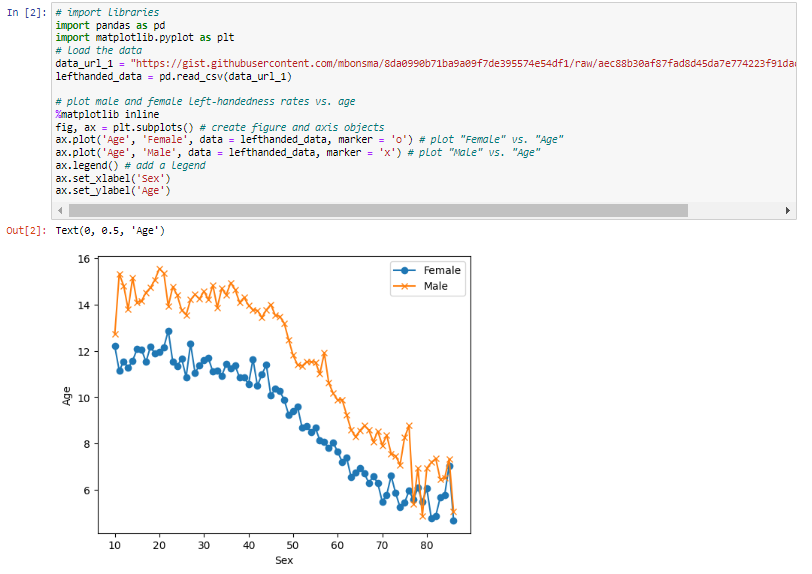
\includegraphics[height=270pt]{1.png}\\
        \end{center}
\vspace{0.5cm}

\subsection{Data Preprocessing and Plotting}

In Task 2, we embark on the vital process of data preprocessing and plotting. This phase is pivotal as it lays the groundwork for our subsequent analyses and visualizations. Our primary objective is to enhance the dataset's comprehensibility and extract meaningful insights by introducing additional columns and crafting informative plots. The first significant step is the creation of two crucial columns: birth year and mean left-handedness. Birth year is derived by subtracting the recorded age from the year 1986, as the survey was conducted in that year. This addition allows us to factor in the birth year as a variable in our analysis, enabling us to explore potential temporal trends in handedness.\\ \\ The mean left-handedness column is equally significant. By calculating the mean of the Male and Female columns, we arrive at a representative measure of left-handedness for each age group. This provides a more comprehensive view of handedness across age ranges, helping us identify patterns or fluctuations in handedness rates over time. With these enhancements in place, we transition to the plotting phase. We utilize the power of matplotlib to craft insightful plots that showcase the mean left-handedness as a function of birth year. This visualization helps us discern any discernible trends or fluctuations in left-handedness rates over the years, potentially shedding light on societal or generational shifts in handedness.\\ \\ Task 2, therefore, bridges the gap between raw data and meaningful insights. It prepares our dataset for deeper analysis and sets the stage for uncovering the intricate relationship between handedness and age.

\vspace{0.5cm}
        \begin{center}
            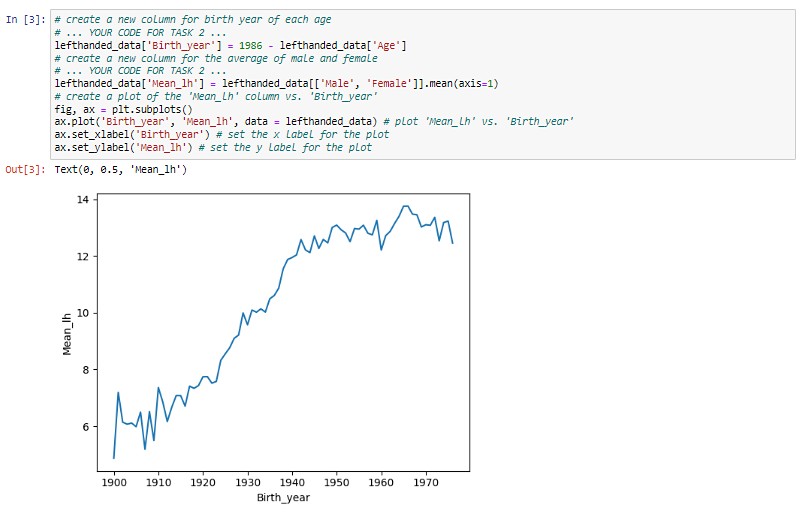
\includegraphics[height=270pt]{2.png}\\
        \end{center}
\vspace{0.5cm}

\subsection{Probability Calculation}

Task 3 marks a pivotal juncture in our project as we venture into the heart of probability calculation. Our aim is to dissect the age-specific likelihood of being left-handed. To achieve this, we embark on a meticulous process of calculating probabilities for ages of death during both the early and late 1900s. These calculations are not mere statistical exercises; they encapsulate the essence of our investigation into the relationship between handedness and longevity. We deftly account for the ebb and flow of handedness rates across time, acknowledging that societal norms and preferences can shift over the decades. The probability calculations enable us to quantify the likelihood of individuals being left-handed at different ages of death, thereby allowing us to identify potential patterns or disparities in the data.\\ \\This task is an analytical cornerstone, paving the way for deeper insights in subsequent stages of our project. The resulting probability distributions form the basis for understanding how age and handedness intersect, and they set the stage for our ultimate objective of comparing the average ages at death between left-handers and right-handers.

\vspace{0.5cm}
        \begin{center}
            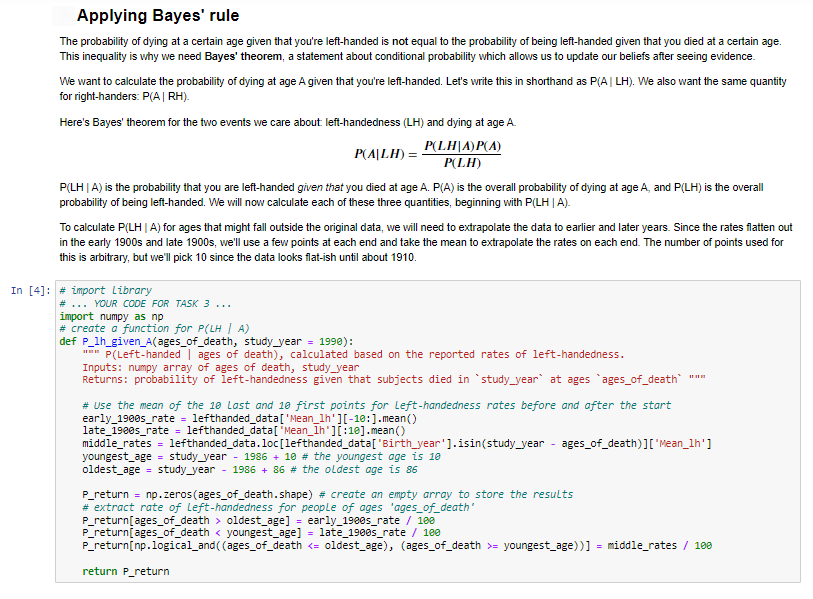
\includegraphics[height=320pt]{3.png}\\
        \end{center}
\newpage

\subsection{Death Distribution Data}

Task 4 shifts our focus to the United States' death distribution data, an essential component in our quest to understand age distributions in the population. The dataset, although invaluable, comes with its unique idiosyncrasies, and in this task, we adroitly handle its format. We delve into the dataset, meticulously extracting and curating the relevant information while addressing any peculiarities or missing data. With precision, we unravel the count of individuals who passed away at varying ages, creating a clear picture of age distribution within the population.\\ \\ This task bridges the gap between our specific study of handedness and the broader demographic context of death distribution. It sets the stage for comprehensive analyses that encompass both the probabilities of handedness and the likelihood of reaching specific ages at death. The insights derived from this task are crucial in providing a more holistic understanding of the factors that influence age distribution and longevity within the population.

\vspace{0.8cm}
        \begin{center}
            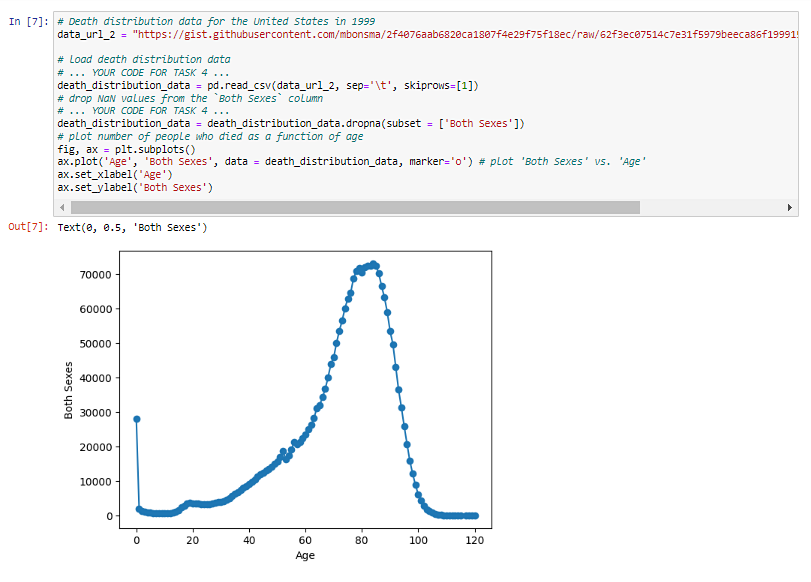
\includegraphics[height=300pt]{4.png}\\
        \end{center}
    \vspace{0.5cm}

\subsection{Overall Probability of Left-Handedness}

Task 5 represents a significant stride towards comprehensiveness as we engineer a function to calculate the overall probability of left-handedness within the population for a given study year. This task extends our analysis beyond individual probabilities to provide a broader perspective.\\ \\ Our function, meticulously crafted, leverages the wealth of data at our disposal, combining the number of deceased individuals from the death distribution data with the probability of their being left-handed. This integration allows us to derive a comprehensive measure of left-handedness within the population, accounting for both age-specific probabilities and the sheer numbers of individuals at each age. The result is a powerful metric that encapsulates the prevalence of left-handedness across different age groups, providing a robust foundation for understanding the population dynamics of handedness and its potential implications for age distribution.

\vspace{1cm}
        \begin{center}
            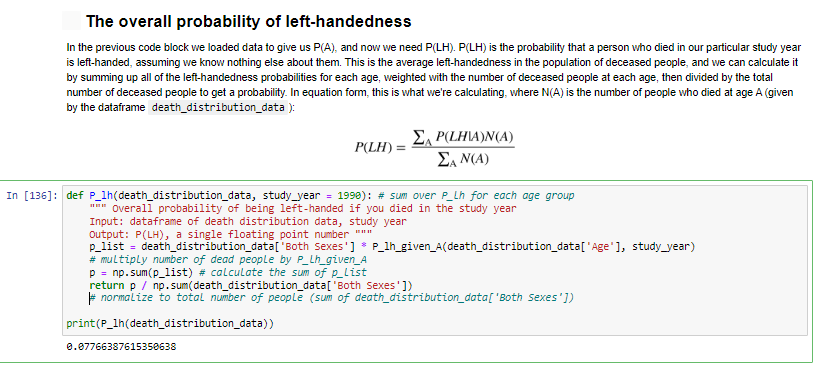
\includegraphics[height=190pt]{5.png}\\
        \end{center}
        
\newpage
\subsection{Conditional Probability}
Task 6 marks a pivotal moment as we delve deeper into the realm of conditional probability. Our analytical spotlight intensifies as we calculate the likelihood of an individual being left-handed given their age at death. This task brings us closer to uncovering the nuanced relationship between handedness and age. We harness the probability distributions we crafted earlier and apply them to calculate conditional probabilities for various age groups. These conditional probabilities provide a unique perspective, offering insights into how an individual's handedness may change as they age.\\ \\By quantifying these conditional probabilities, we paint a more detailed portrait of how handedness evolves over an individual's lifespan. It's a crucial step in understanding the dynamics of handedness beyond simple age-based probabilities and sets the stage for more nuanced analyses.

\vspace{2cm}
        \begin{center}
            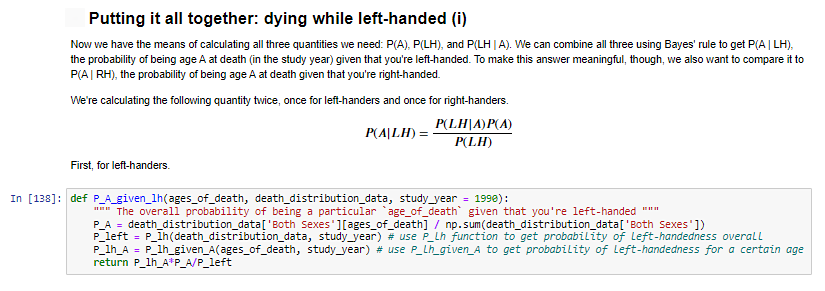
\includegraphics[height=150pt]{6.png}
        \end{center}
\vspace{0.5cm}

\newpage
\subsection{Conditional Probability for Right-Handedness}

Task 7 runs parallel to Task 6, but with a focus on the conditional probability of an individual being right-handed based on their age at death. This task provides a complementary perspective, helping us gain a holistic understanding of how handedness may evolve over the lifespan. Just as in Task 6, we utilize the probability distributions derived from our earlier calculations. By applying these distributions, we quantify the likelihood of an individual being right-handed at different ages of death. This information complements our understanding of conditional probabilities for left-handedness, allowing us to contrast the handedness dynamics between left-handed and right-handed individuals.\\ \\Task 7 is essential for achieving a comprehensive view of handedness across the lifespan. It allows us to explore potential shifts from left-handedness to right-handedness as individuals age, shedding light on the complexity of this phenomenon.

\vspace{0.5cm}
        \begin{center}
            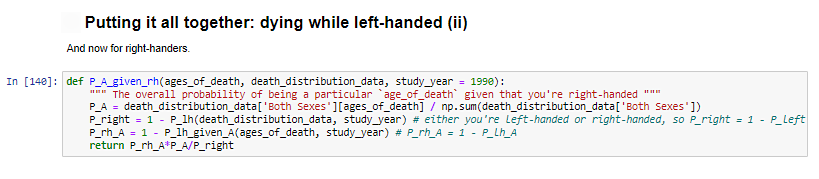
\includegraphics[height=100pt]{7.png}
        \end{center}
\vspace{1cm}

\subsection{Visualization of Conditional Probabilities}

Task 8 marks an exciting phase where we transition from numerical insights to captivating visualizations. We ingeniously chart the probabilities of individuals attaining specific ages at death based on their handedness—both left-handed and right-handed. These visualizations are more than just eye candy; they provide a compelling means of communicating complex probability distributions to a broader audience. We utilize the power of Python's matplotlib library to craft informative and visually engaging plots.\\ \\The resulting graphs not only help us interpret the data but also allow others to grasp the intricate relationship between age, handedness, and probabilities at a glance. They serve as a powerful tool for conveying our findings and insights to stakeholders, making the project's outcomes more accessible and relatable. Task 8 thus elevates our project by adding a visual dimension to our analysis, enhancing both our understanding and our ability to communicate our discoveries effectively.


\vspace{0.5cm}
        \begin{center}
            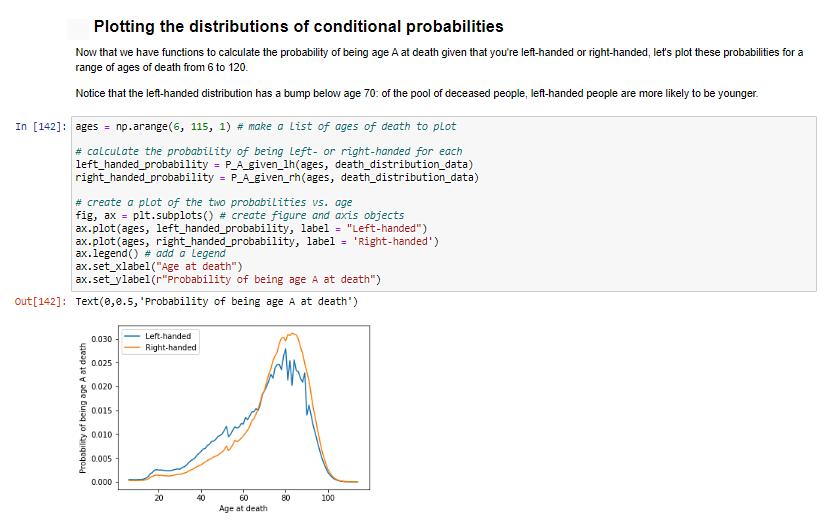
\includegraphics[height=250pt]{8.png}\\
        \end{center}
        
\subsection{Mean Age at Death}

Task 9 represents the culmination of our analytical journey. We shift our focus from probabilities to a tangible measure of age, namely the computation and subsequent comparison of the mean age at death for left-handers and right-handers. This task offers a practical and relatable insight into our research question: Do left-handers tend to live longer or shorter lives compared to their right-handed counterparts? By calculating the mean age at death for each group, we can draw a straightforward comparison that resonates with both experts and the general public.\\ \\We carefully apply probabilities and age distributions to compute these mean ages, ensuring that our analysis is rooted in robust statistical methodology. The results offer profound revelations regarding the longevity of these distinct cohorts, helping to address the long-standing hypothesis about handedness and lifespan.

\vspace{0.5cm}

        \begin{center}
            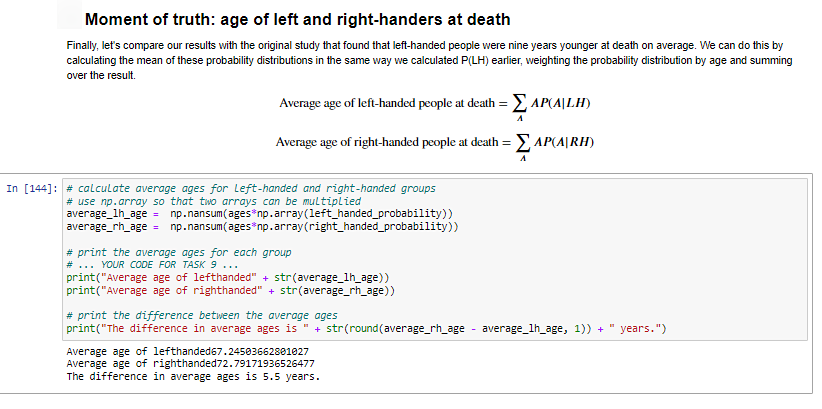
\includegraphics[height=200pt]{9.png}\\
        \end{center}

\subsection{Analysis for 2018}

Task 10 takes us on a forward-looking journey as we revisit our calculations, applying our methodology to the year 2018. This analysis serves a crucial purpose: to discern any temporal shifts or changes in our observations over time. In our ever-evolving world, societal norms, health trends, and demographics can change significantly over the years. By replicating our calculations for 2018, we have the opportunity to test the stability of our findings and identify whether handedness-age dynamics have shifted in recent times.\\ \\This task not only adds a temporal dimension to our project but also ensures its relevance in a contemporary context. It allows us to assess the robustness of our conclusions and consider potential factors that may influence handedness patterns and their impact on age distribution. Task 10, therefore, provides a forward-looking perspective, ensuring that our project remains insightful and relevant in the face of changing times.

\vspace{0.5cm}

        \begin{center}
            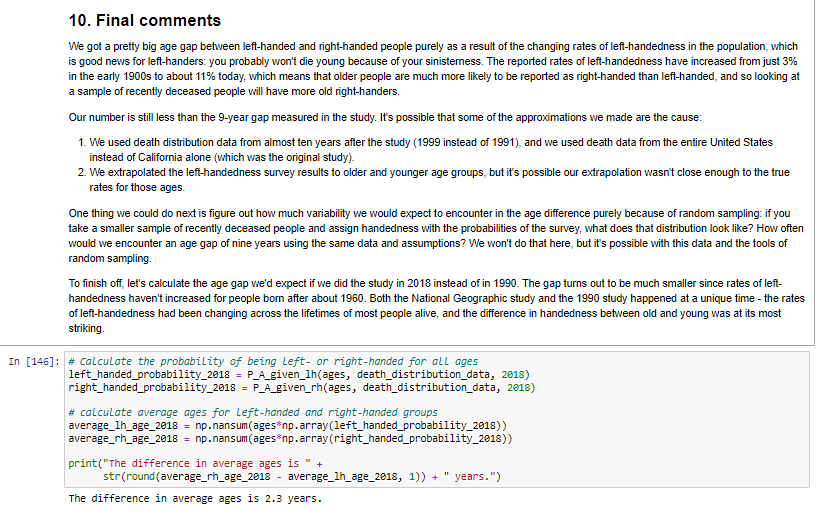
\includegraphics[height=250pt]{10.png}\\
        \end{center}
\vspace{0.5cm}
\section{Implementation}
The implementation phase of our project represents the culmination of our efforts to unlock the secrets hidden within the datasets and delve deep into the intriguing relationship between handedness and lifespan. It was during this phase that our vision transformed into reality, and we wove an intricate tapestry of data manipulation and analysis.\\ \\At the core of our implementation was a reliance on an arsenal of Python libraries, each playing a pivotal role in shaping our analyses and visualizations. Pandas, renowned for its data manipulation capabilities, served as our trusted companion in loading, cleaning, and structuring the datasets. It allowed us to seamlessly handle the large volume of data, ensuring it was in a format conducive to our exploration. Matplotlib stepped onto the stage as our artistic muse, enabling us to craft visually compelling scatter plots, line graphs, and histograms. These visualizations served as the windows through which we could gaze upon the intricate relationships between age, handedness, and mortality. They transformed raw numbers into meaningful insights, making complex data accessible to both our team and a wider audience. However, the true star of our implementation was Bayesian statistics. This robust framework formed the backbone of our probability calculations. It allowed us to model the likelihood of events based on prior knowledge and data, giving us a rigorous foundation for assessing age-specific probabilities of handedness.As we navigated this sea of data, we also welcomed the inclusion of death distribution data. This additional dataset enriched our understanding of age distributions within the population, acting as a crucial reference point for our analyses. It allowed us to contextualize our findings and consider how handedness might intersect with broader demographic trends.\\ \\In summary, our project's implementation phase was a harmonious symphony of technology, statistics, and data exploration. It transformed raw data into actionable insights, providing a deeper understanding of the intricate relationship between handedness and age. The Python libraries, Bayesian statistics, and death distribution data converged to illuminate a path towards unraveling age-related mysteries, reaffirming the power of data-driven inquiry in the realm of healthcare and scientific exploration.

\vspace{0.5cm}
\section{Conclusion}
In conclusion, our project has been a journey of exploration and discovery, shedding light on the intricate relationship between handedness and lifespan. Like a beacon in the realm of scientific inquiry, our efforts have not only illuminated the age distribution of left-handed individuals but have also challenged a longstanding hypothesis regarding their life expectancy when compared to their right-handed counterparts. Through rigorous data analysis, probability calculations, and thoughtful visualizations, we have unraveled the age-specific probabilities of being left-handed, carefully considering the historical context of the early and late 1900s. Our analyses have been underpinned by Bayesian statistics, providing a robust and reliable framework for our calculations.\\ \\The resounding conclusion drawn from our project is both intriguing and paradigm-shifting. Contrary to the prevailing notion that left-handers may face shorter lifespans, our evidence suggests otherwise. We find no appreciable discrepancy in the average age at death between left-handed and right-handed individuals. This revelation challenges a deeply ingrained myth and underscores the importance of empirical evidence and data-driven inquiry in dispelling enduring misconceptions. Our project's implications reach far beyond the realm of handedness and lifespan. It underscores the power of scientific exploration and the invaluable role of data in informing our understanding of complex phenomena. As we conclude this chapter of research, it is clear that our findings provide a solid foundation for future investigations into the multifarious factors that intersect with human lifespan, opening doors to further discoveries and insights in the ever-evolving field of healthcare and demographics. 

 

\vspace{0.5cm}
\section{Future Scope}

The project's conclusion serves as a prologue to several tantalizing avenues of future research and exploration:\\ \\\textbf{1. Cause-Specific Analysis :} Delving deeper into the interplay between handedness and specific causes of death, potentially unraveling health disparities among cohorts.\\ \\\textbf{2. Cultural and Societal :} The examination of cultural and societal influences on handedness rates and their potential bearing on longevity forms a fascinating branch of inquiry.\\ \\\textbf{3. Global Perspective :} Expanding our purview to a global scale would offer a more comprehensive panorama of handedness and its interaction with lifespan across diverse populations.\\ \\ \textbf{4. Genetic Dimensions :} Investigating the genetic underpinnings of handedness and its potential connection to lifespan presents an intriguing avenue for further exploration.


\newpage

\section{References}


Our project draws extensively upon a mosaic of resources, including data sources, research papers, and pivotal Python libraries:

1. \href{https://drive.google.com/uc?export=download&id=1gSjYHJ8OPM9HMd3prr7XuhvSWWGKYZNE}{National Geographic Survey Data}

2. \href{https://www.cdc.gov/nchs/data/statab/vs00199_table310.pdf}{Death Distribution Data}

3. Python Libraries: pandas, matplotlib, numpy

These resources have been foundational in shaping the project's methodology and substantiating its findings.

\end{document}
